\section{Aukro.cz}

\label{analyza:aukro}

Webová aplikace Aukro.cz \cite{aukro} se nezabývá jen aukcemi, ale také klasickým prodejem zboží. Protože je to ve své podstatě e-shop, očekávám dobře zvolené kategorie, detaily v~popise zboží a v~případě Aukra i výrazné zobrazení hodnocení prodejců zboží.

\subsection{Hlavní stránka}
Viz obrázek \ref{fig:aukro:home}.
\begin{figure}[h]
    \centering
    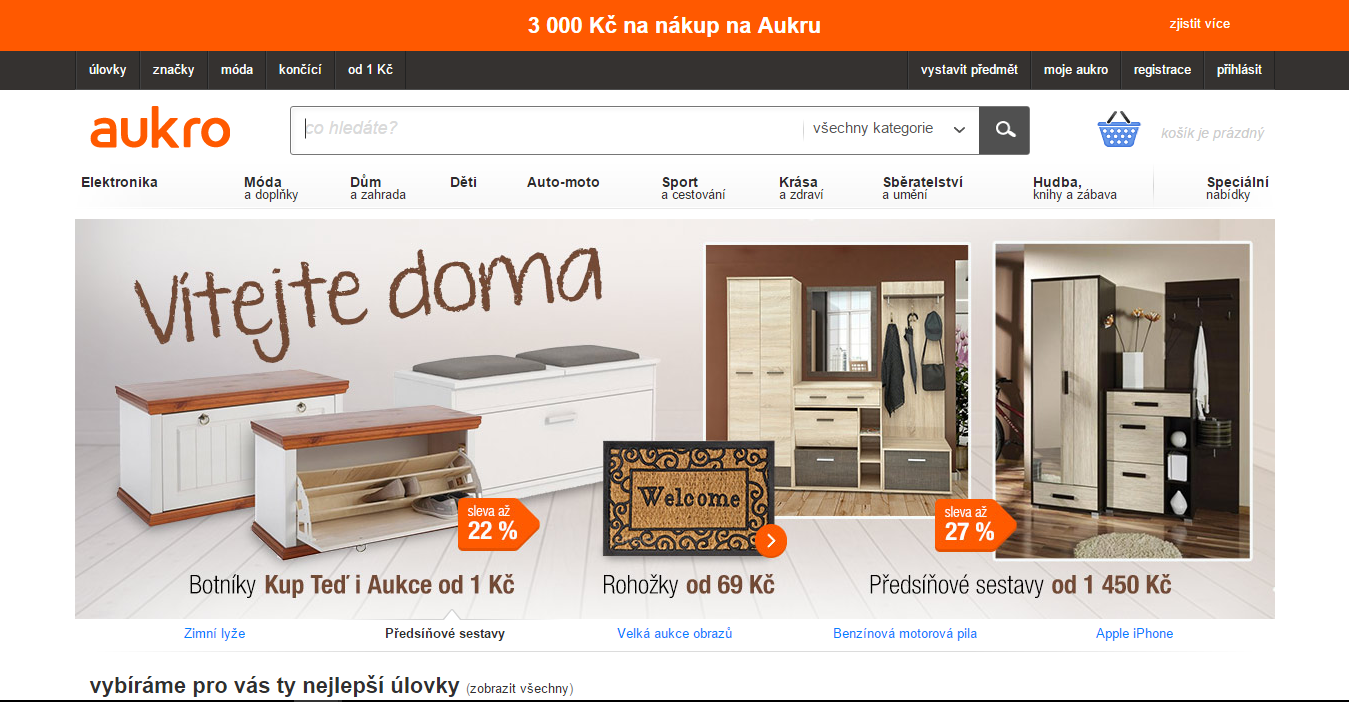
\includegraphics[width=1.0\textwidth]{media/aukro/home.png}
    \caption{Aukro.cz -- Hlavní stránka}
    \label{fig:aukro:home}
\end{figure}
\subsubsection*{Pozitiva}
\begin{itemize}
    \item[+] \textbf{Co hledáte?} -- Nejdůležitější prvek (vyhledávání) úvodní stránky je dostatečně velký a je na místě, kde ho uživatelé očekávají.
    \item[+] \textbf{Kategorie} -- Při najetí myší se kromě podkategorií zobrazí i populární kategorie a jedna speciální nabídka zboží. To může mít za důsledek to, že si uživatelé nakoupí i něco, co předtím nechtěli, nebo to nebylo jejich prioritou.
\end{itemize}
\subsubsection*{Negativa}
\begin{itemize}
    \item[-] \textbf{Poutač} -- Velký poutač na speciální akce Aukra. Pokud chce uživatel vidět nějaké zboží, které mu vybralo Aukro, nebo naposledy prohlédnuté zboží, tak musí přejít poměrně dlouhý kus stránky.
\end{itemize}


%%%%%%%%%%%%%%%%%%%%%%%%%%%%%%%%%%%%%%%%%%%%%%%%%%%%%%%%%%%%%%%%%%%%%%%%%%%%%%%%%%%%%%%%%%%%%%%%%%%%%%%%%%%%%%%%%%%%%%%%

\newpage
\subsection{Vyhledávání zboží}
Viz obrázek \ref{fig:aukro:search}.
\begin{figure}[h]
    \centering
    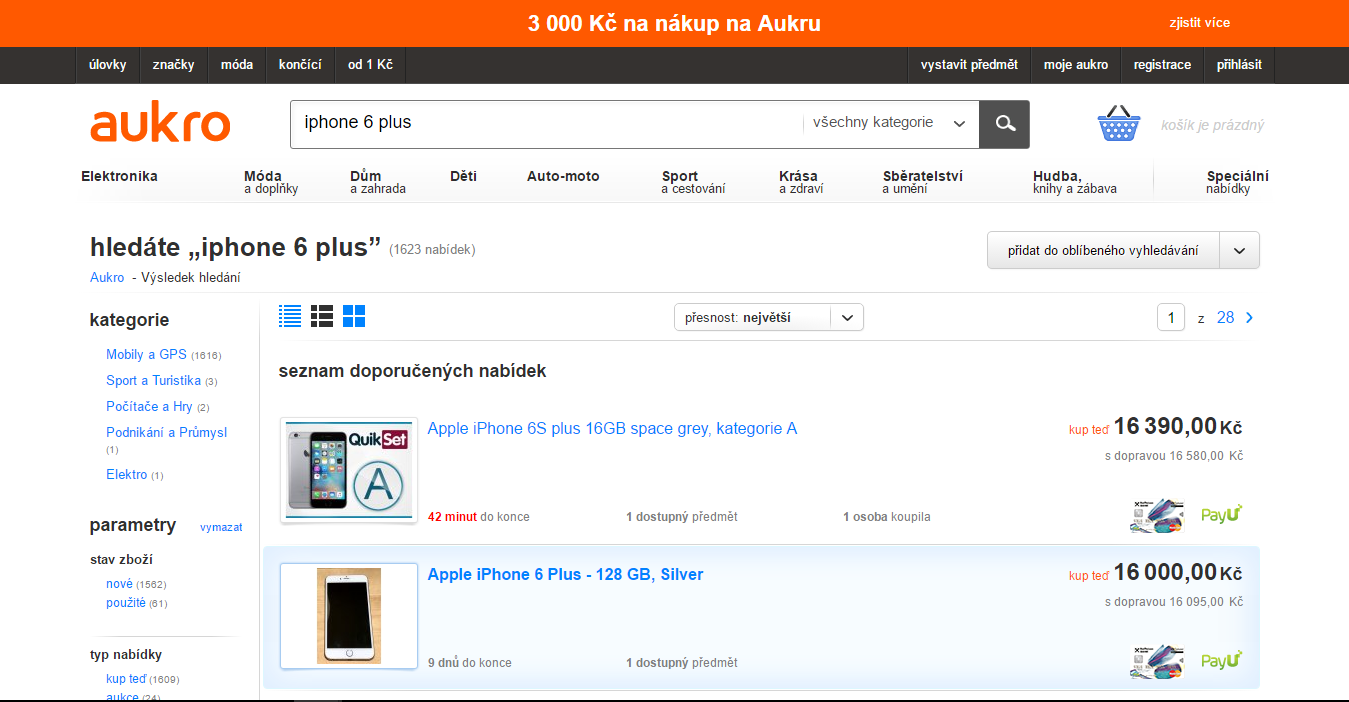
\includegraphics[width=1.0\textwidth]{media/aukro/search.png}
    \caption{Aukro.cz -- Vyhledávání zboží}
    \label{fig:aukro:search}
\end{figure}
\subsubsection*{Pozitiva}
\begin{itemize}
    \item[+] \textbf{Cena i s~dopravou} -- Na stránce je přímo zobrazena cena i s~dopravou. Uživatel cítí určitou transparentnost a nemusí si tyto informace vyhledávat sám.
\end{itemize}
\subsubsection*{Negativa}
\begin{itemize}
    \item[-] \textbf{Málo informací o~zboží} -- O~konkrétním zboží se člověk kromě názvu moc nedozví. Místo na alespoň pár detailů tam přitom existuje.
    \item[-] \textbf{Málo nabídek} -- Dvě nabídky zaberou celou stránku ve výchozím nastavení.
    \item[-] \textbf{Chaotické rozhraní} -- Rozhraní je chaotické a neuspořádané.
\end{itemize}


%%%%%%%%%%%%%%%%%%%%%%%%%%%%%%%%%%%%%%%%%%%%%%%%%%%%%%%%%%%%%%%%%%%%%%%%%%%%%%%%%%%%%%%%%%%%%%%%%%%%%%%%%%%%%%%%%%%%%%%%

\newpage
\subsection{Detail zboží}
Viz obrázek \ref{fig:aukro:detail}.
\begin{figure}[h]
    \centering
    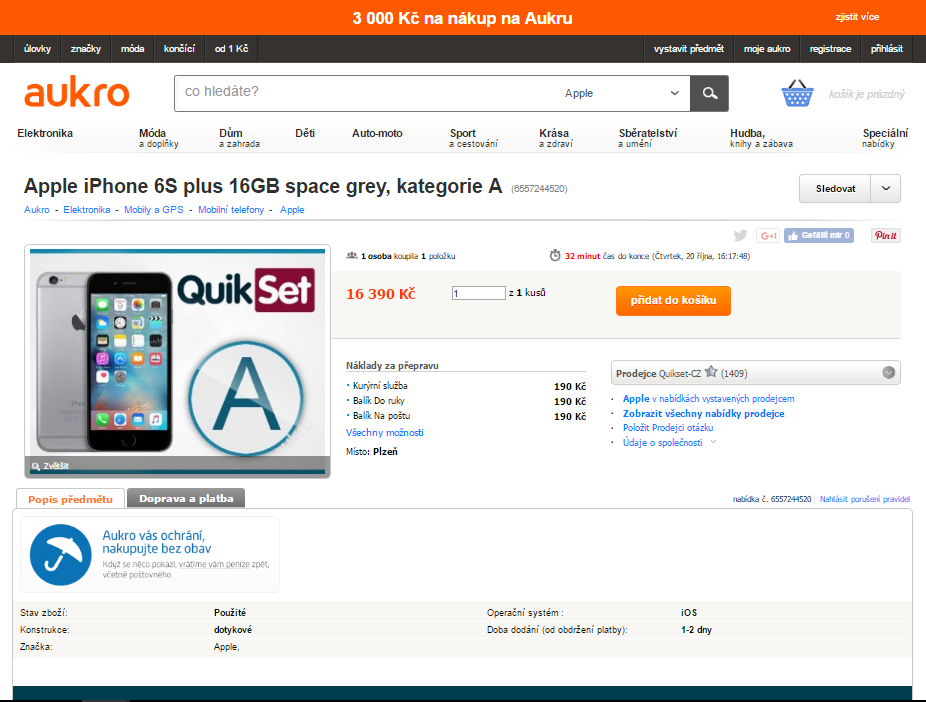
\includegraphics[width=1.0\textwidth]{media/aukro/detail.png}
    \caption{Aukro.cz -- Detail zboží}
    \label{fig:aukro:detail}
\end{figure}
\subsubsection*{Negativa}
\begin{itemize}
    \item[-] \textbf{Neobsahuje moc detailů} -- Detaily se nacházejí až ve spodní části stránky.
    \item[-] \textbf{Hodnocení prodejců} -- Sice se hodnocení prodejců na stránce nachází, ale výrazně je viditelnější až po rozkliknutí.
    \item[-] \textbf{Chaotické rozhraní} -- Problém uživatelského rozhraní zůstává.
\end{itemize}


%%%%%%%%%%%%%%%%%%%%%%%%%%%%%%%%%%%%%%%%%%%%%%%%%%%%%%%%%%%%%%%%%%%%%%%%%%%%%%%%%%%%%%%%%%%%%%%%%%%%%%%%%%%%%%%%%%%%%%%%

\newpage
\subsection{Profil prodejce}
Viz obrázky \ref{fig:aukro:profile} a  \ref{fig:aukro:profile2}.
\begin{figure}[h]
    \centering
    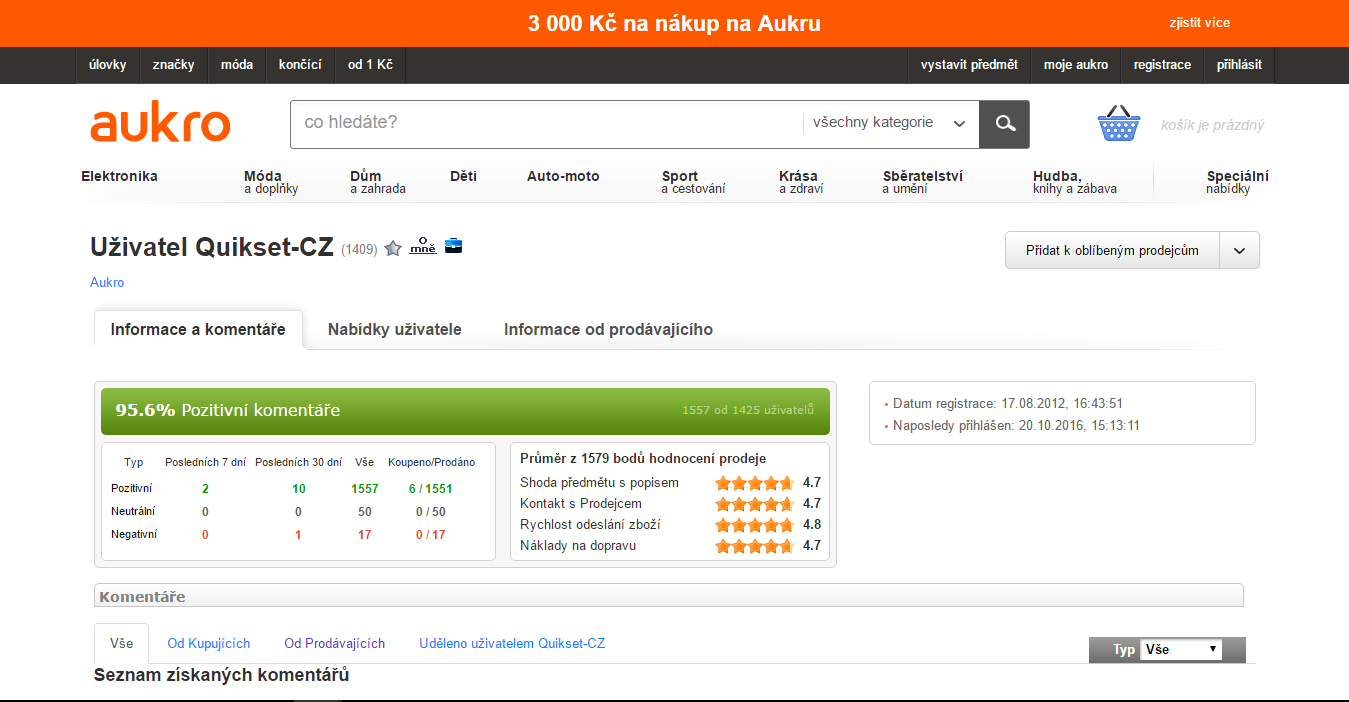
\includegraphics[width=1.0\textwidth]{media/aukro/profile.png}
    \caption{Aukro.cz -- Profil prodejce}
    \label{fig:aukro:profile}
\end{figure}
\begin{figure}[h]
    \centering
    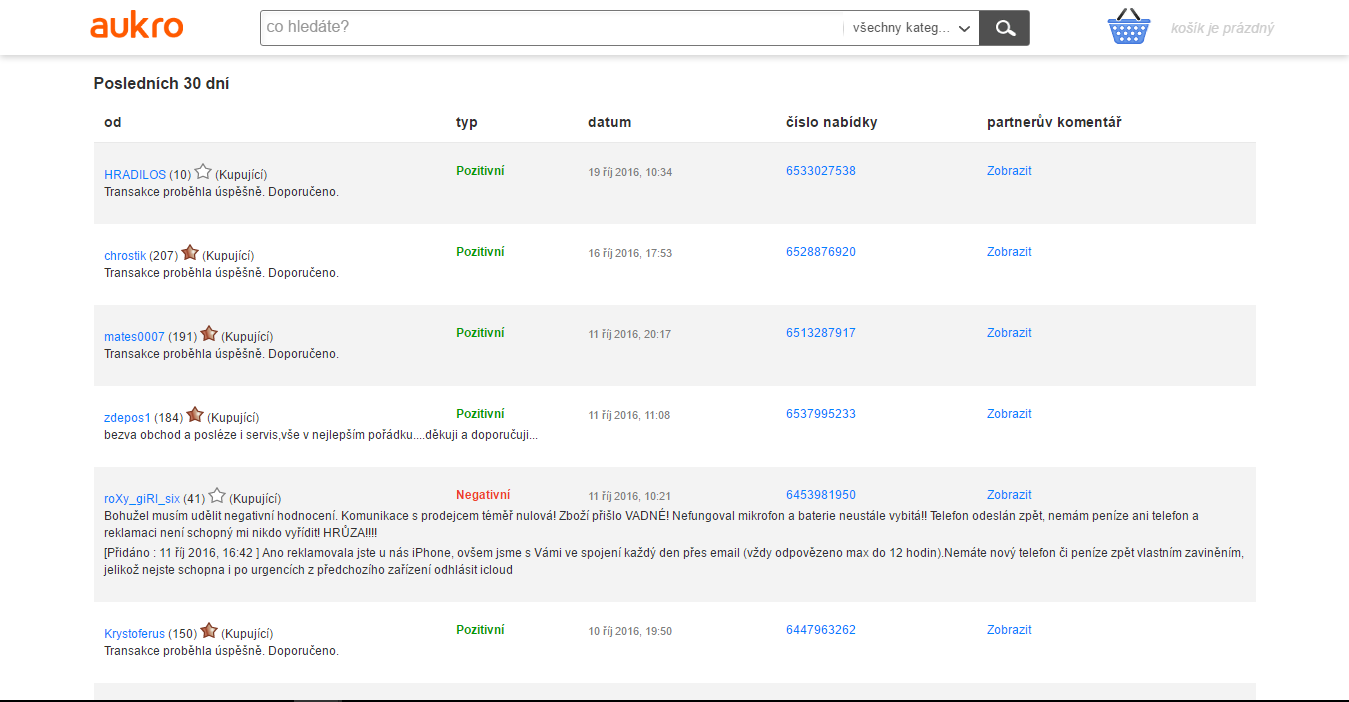
\includegraphics[width=1.0\textwidth]{media/aukro/profile2.png}
    \caption{Aukro.cz -- Recenze uživatele}
    \label{fig:aukro:profile2}
\end{figure}
\subsubsection*{Pozitiva}
\begin{itemize}
    \item[+] \textbf{Historie hodnocení/komentářů} -- Možnost přečíst si kdo byl jak spokojený s~daným prodejcem.
\end{itemize}
\subsubsection*{Negativa}
\begin{itemize}
    \item[-] \textbf{Nepřehlednost} -- Problémy s~rozhraním se projevují i na této stránce. Nedá se vytvořit si závěry bez dlouhého posouvání se na stránce.
\end{itemize}


%%%%%%%%%%%%%%%%%%%%%%%%%%%%%%%%%%%%%%%%%%%%%%%%%%%%%%%%%%%%%%%%%%%%%%%%%%%%%%%%%%%%%%%%%%%%%%%%%%%%%%%%%%%%%%%%%%%%%%%%

\subsection{Shrnutí}
Při analyzování Aukro.cz jsem narazil na tyto nedostatky:
\begin{itemize}
    \item \textbf{chaotické rozhraní},
    \item \textbf{nedetailnost},
    \item \textbf{málo poskytnutých informací}.
\end{itemize}

Z~pohledu této práce se jeví být důležitou funkcí \textbf{historie komentářů}, kdy si uživatel může vytvořit názor o~prodejci. Je však nutné, aby uživatelské rozhraní bylo přehledné a určitě aby poskytovalo všechny potřebné detaily. To pro tuto práci znamená: jaká je daná nabídka, jak daleko je vzdálená a jaké hodnocení má prodejce -- a to vše na jednom místě.